\documentclass{beamer}
\usepackage[utf8]{inputenc}
\usepackage{xeCJK} 
\usepackage[T1]{fontenc}
\usepackage{mathabx}
\usepackage{amsmath} 
\usepackage{mathpazo}
\usepackage{bibentry}
\usepackage{tikz}
\usepackage{caption}
\usepackage{graphicx, subfig}

\usetikzlibrary{scopes}
\def\iangle{35} % Angle of the inclined plane
\def\down{-90}
\def\arcr{0.5cm} % Radius of the arc used to indicate angles

\usetheme{Boadilla}
\usecolortheme{wolverine}
\useoutertheme{miniframes}

\title{VP160 Recitation Class III}
\author{Zeyi Ren}
\institute{UM-SJTU Joint Institute}

\begin{document}

\maketitle

\frame{\tableofcontents}

\section{Force \& Inertial FoR}
\begin{frame}{Force and Inertial Frame of Reference}
  \begin{block}{Force}
    Force represents \textbf{interaction} between two objects or an object and its environment. 
  \end{block}
  Two types of forces:\\
  \begin{itemize}
    \item Contact forces: objects are in contact with each other and exert forces on each other.\\ \textcolor{blue}{e.g.} force of friction
    \item Non-contact (field) forces: objects are not in contact with each other and exert forces on each other.\\ \textcolor{blue}{e.g.} gravitational force
  \end{itemize}
\end{frame}

\begin{frame}
  \begin{block}{Inertial frame of reference}
     In an inertial FoR, a physical object with zero net force acting on it moves with a constant velocity (which might be zero), or, equivalently, it is a frame of reference in which Newton's first law of motion holds.
  \end{block}
\end{frame}

\section{Newton's Law}
\begin{frame}{Newton's Law}
  \begin{block}{Newton's First Law}
    An object at rest will stay at rest, and an object in motion will stay in motion unless acted on by a net external force.
  \end{block}
  $$
  \sum{\vec{F}} = 0 \Leftrightarrow \vec{a} = 0
  $$

  \begin{block}{Newton's Second Law}
    In an inertial frame of reference, acceleration of a particle is directly proportional to the net force acting upon it, and inversely proportional to its mass.
  \end{block}
  $$
  \vec{F} = m\vec{a}
  $$
\end{frame}

\begin{frame}
  Using Newton's second law, normally we can derive the equation of motion:
  $$\frac{d^2r}{dt^2}=\frac{F(\dot{r},r,t)}{m}$$ with $v(t_0) = v_0, r(t_0) = r_0$ known, it's an initial value problem to be solved.\\\textcolor{blue}{How to solve initial value problem?}
  \begin{block}{Newton's Third Law}
    The mutual forces of action and reaction between two bodies are equal in magnitude and opposite in direction.
  \end{block}
  $$
  \vec{F_1} = -\vec{F_2}
  $$
\end{frame}

\section{Free-body Diagram}
\begin{frame}
  \begin{block}{Free-body diagram}
    A free body diagram consists of a diagrammatic representation of a single body or a subsystem of bodies isolated from its surroundings showing all the forces acting on it.
  \end{block}
  Normally, you need to consider:
  \begin{enumerate}
    \item Normal force
    \begin{itemize}
      \item direction: perpendicular to the surface.
    \end{itemize}
    \item Friction force
    \begin{itemize}
      \item cause: normal force
      \item direction: in the opposite of $\vec{v}$.
    \end{itemize}
    \item Tension force
    \begin{itemize}
      \item direction: along the rope/rod/spring.
    \end{itemize}
    \item Weight
  \end{enumerate}
\end{frame}

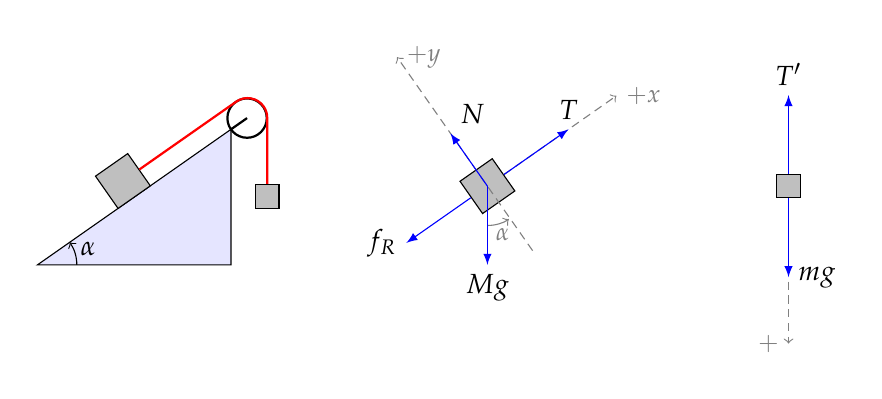
\begin{tikzpicture}[
  force/.style={>=latex,draw=blue,fill=blue},
  axis/.style={densely dashed,gray,font=\small},
  M/.style={rectangle,draw,fill=lightgray,minimum size=0.5cm,thin},
  m/.style={rectangle,draw=black,fill=lightgray,minimum size=0.3cm,thin},
  plane/.style={draw=black,fill=blue!10},
  string/.style={draw=red, thick},
  pulley/.style={thick},
]

\matrix[column sep=1cm] {
  %% Sketch
  \draw[plane] (0,-1) coordinate (base)
                   -- coordinate[pos=0.5] (mid) ++(\iangle:3) coordinate (top)
                   |- (base) -- cycle;
  \path (mid) node[M,rotate=\iangle,yshift=0.25cm] (M) {};
  \draw[pulley] (top) -- ++(\iangle:0.25) circle (0.25cm)
                 ++ (90-\iangle:0.5) coordinate (pulley);
  \draw[string] (M.east) -- ++(\iangle:1.5cm) arc (90+\iangle:0:0.25)
                -- ++(0,-1) node[m] {};

  \draw[->] (base)++(\arcr,0) arc (0:\iangle:\arcr);
  \path (base)++(\iangle*0.5:\arcr+5pt) node {$\alpha$};
  %%

&
  %% Free body diagram of M
  \begin{scope}[rotate=\iangle]
      \node[M,transform shape] (M) {};
      % Draw axes and help lines

      {[axis,->]
          \draw (0,-1) -- (0,2) node[right] {$+y$};
          \draw (M) -- ++(2,0) node[right] {$+x$};
          % Indicate angle. The code is a bit awkward.

          \draw[solid,shorten >=0.5pt] (\down-\iangle:\arcr)
              arc(\down-\iangle:\down:\arcr);
          \node at (\down-0.5*\iangle:1.3*\arcr) {$\alpha$};
      }

      % Forces
      {[force,->]
          % Assuming that Mg = 1. The normal force will therefore be cos(alpha)
          \draw (M.center) -- ++(0,{cos(\iangle)}) node[above right] {$N$};
          \draw (M.west) -- ++(-1,0) node[left] {$f_R$};
          \draw (M.east) -- ++(1,0) node[above] {$T$};
      }

  \end{scope}
  % Draw gravity force. The code is put outside the rotated
  % scope for simplicity. No need to do any angle calculations. 
  \draw[force,->] (M.center) -- ++(0,-1) node[below] {$Mg$};
  %%

&
  %%%
  % Free body diagram of m
  \node[m] (m) {};
  \draw[axis,->] (m) -- ++(0,-2) node[left] {$+$};
  {[force,->]
      \draw (m.north) -- ++(0,1) node[above] {$T'$};
      \draw (m.south) -- ++(0,-1) node[right] {$mg$};
  }

\\
};
\end{tikzpicture}

\begin{frame}
\textcolor{red}{Background}\\
Statics and particles in equilibrium:\\
$$
  \sum{\vec{F}} = 0%\Rightarrow  \left\{
  %   \begin{aligned}
  %   \sum{F_x} & =  0 \\
  %   \sum{F_y} & =  0 \\
  %   \sum{F_z} & =  0
  %   \end{aligned}
  %   \right.  
$$

\section{Application of Newton's Law}
\textcolor{blue}{Exercise 1}\\
\textcolor{blue}{\footnotesize{Application of free-body diagram and \textcolor{red}{"Isolation Method"}}}\\
Two identical smooth balls $A$ and $B$ are suspended from a fixed point $O$ by two ropes of the same length. The two balls also support a smooth ball $C$ of the same weight with A and B, as shown in the Fig. The system are now at an equilibrium. \textbf{Find} the relationship between $\alpha$ and $\beta$.
\end{frame}

\begin{frame}
  \begin{figure}[H]
    \centering
    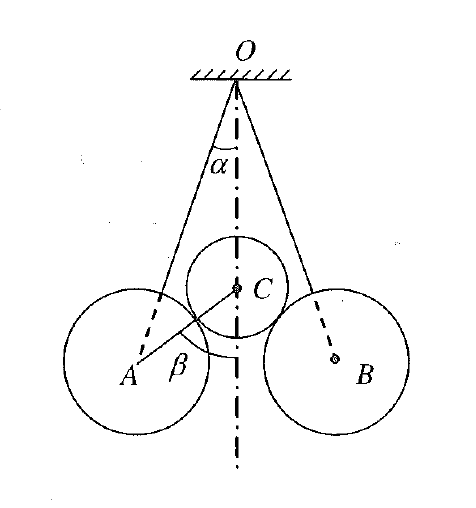
\includegraphics[width=0.4 \linewidth, angle =0]{ex1.png}
    % \caption{.}
    \begin{center}
      Figure 1. Exercise 1.
    \end{center}
    \label{fig:4}
    \end{figure}
\end{frame}

\begin{frame}
\textcolor{blue}{Exercise 2}\\
\textcolor{blue}{\footnotesize{Force of friction and \textcolor{red}{"Whole Method"}}}\\

Two blocks with mass $m_1$ and $m_2$ are stacked on the horizontal desk. Another block with mass $m$ connected to $m_1$ and $m_2$ with an inextensible rope is put onto a pulley system. The system is showed in Fig.2. Suppose the friction coefficient between $m_1$ and $m_2$ is $\mu$, and the desk is smooth enough to neglect friction. \textbf{Find:}\\ 
What conditions does the system need to satisfy if there is no relative sliding between $m_1$ and $m_2$.
\begin{figure}[htbp]
\centering
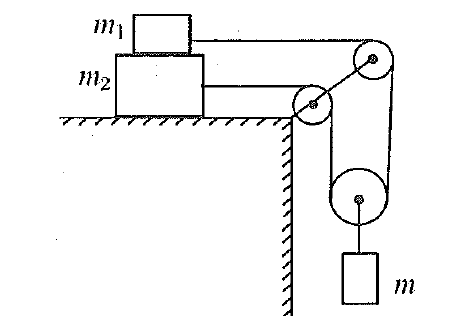
\includegraphics[width=0.35 \linewidth, angle =0]{ex2.png}
% \caption{.}
\begin{center}
  Figure 2. Exercise 2.
\end{center}
\label{fig:2}
\end{figure}
\end{frame} 

\begin{frame}
\textcolor{blue}{Exercise 3}

Mass $m$ hangs on a massless rope in a car moving with\\ 
(a) constant velocity \textbf{v},\\
(b) constant acceleration \textbf{a}\\
on a horizontal surface. What is the angle the rope forms with the vertical direction.\\
Discuss the problems (a) (b) if the car slides (without friction) down a plane inclined at an angle $\alpha$.
\end{frame}

\begin{frame}
\textcolor{blue}{Exercise 4}

A monkey with mass $m$ holds a rope hanging over a frictionless pulley attached to mass $M$ (see
figure). Discuss motion of the system if the monkey\\
(a) does not move with respect to the rope,\\
(b) climbs up the rope with constant velocity $\mathbf{v_0}$ with respect to the rope,\\
(c) climbs up the rope with constant acceleration $\mathbf{a_0}$ with respect to the rope.
\begin{figure}[htbp]
\centering
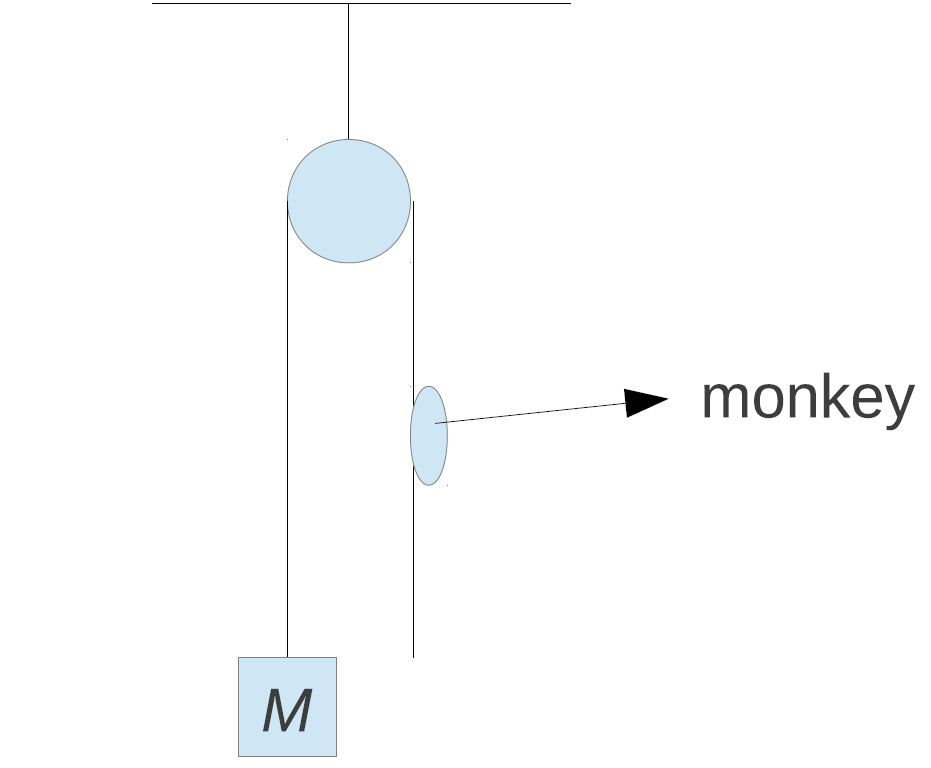
\includegraphics[width=0.4 \linewidth, angle =0]{ex4.png}
% \caption{Exercise 2.}
\label{fig:4}
\end{figure}
\end{frame}

\begin{frame}
\textcolor{blue}{Exercise 5}\\
\textcolor{blue}{\footnotesize{Relative Motion and Newton's Second law}}\\

See in Fig.1, a split ABC with mass $M$, height $h$ is placed on the horizontal plane. The inclination angle of AC is $\theta$. A small object with mass $m$ begin to slide down from A with initial velocity 0. Omitting the friction of each contact surface. \textbf{find}:\\
(a) The displacement of $M$ when $m$ reaches the ground,\\
(b) in the ground FoR, the acceleration $\mathbf{a_1}$ of $M$.\\
(c) in the $m$ FoR(small object), the acceleration $\mathbf{a_2'}$ of $M$,\\
(d) in the ground FoR, the acceleration $\mathbf{a_2}$ of $m$,\\
(e) the normal force $N$ between $m$ and $M$,\\
(f) the normal force $R$ between $M$ and the ground.
\end{frame}

\begin{frame}
  \begin{figure}[htbp]
    \centering
    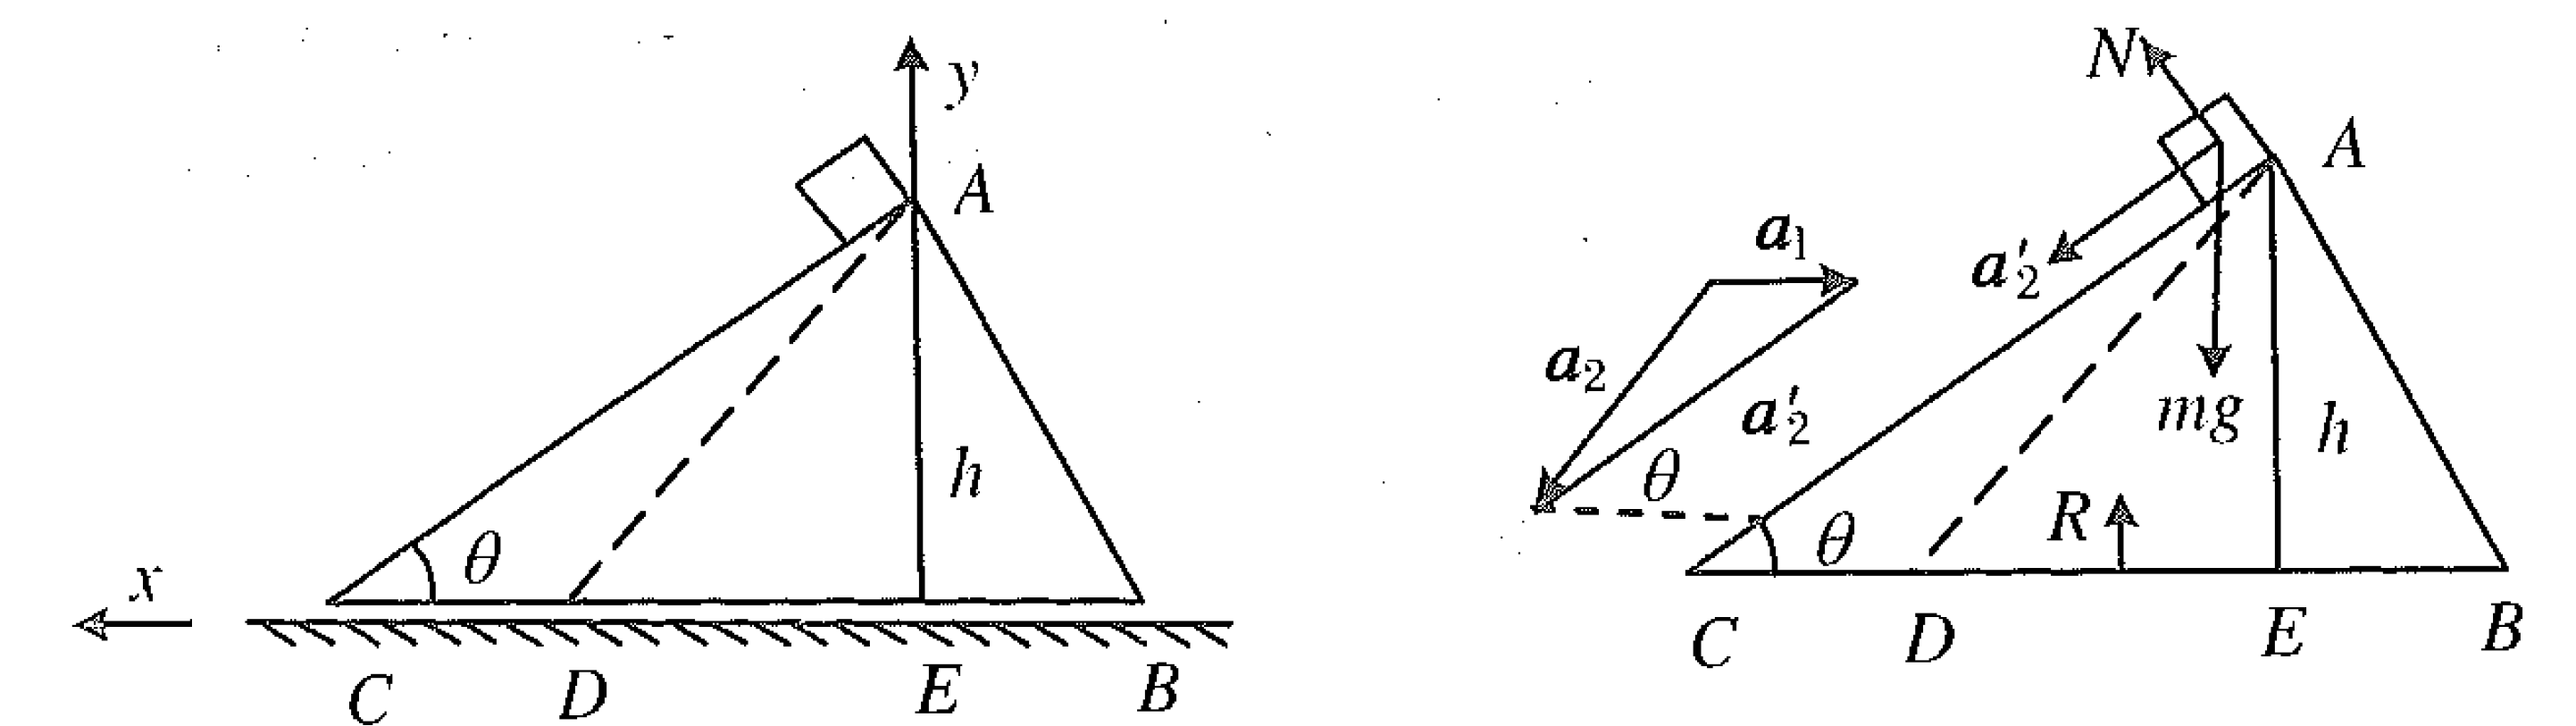
\includegraphics[width=1 \linewidth, angle =0]{ex5.png}
    % \caption{Exercise 3.}
    \begin{center}
      Figure 4. Exercise 5.
      \end{center}
    \label{fig:5}
    \end{figure}
\end{frame}

\section{Motion with Drag}
\begin{frame}{Motion with Air/Fluid Drag}
  Consider a particle with linear drag $\mathbf{F} = -k\mathbf{v}$ and initial velocity $\mathbf{v_0} = v_0cos(\alpha)\hat{n_x} + v_0sin(\alpha)\hat{n_y}$, what's its trajectory? \\
  ~\\
  \textcolor{blue}{Two recommended ways:}\\
  \begin{enumerate}
    \item decompose the drag force
    \item decompose the velocity
  \end{enumerate}
  ~\\
  What if quadratic drag force?
\end{frame}

% \section{Simple Harmonic Motion}
% \begin{frame}
%   q
% \end{frame}

\begin{frame}{Reference}
  \begin{thebibliography}{9}
  \setbeamertemplate{bibliography item}[article]
  \bibitem{C} Yigao Fang.\\
  \textcolor{black}{VP160 Recitation Slides.}\\
  2020
  \bibitem{C} Haoyang Zhang.\\
  \textcolor{black}{VP160 Recitation Slides.}\\
  2020
  \setbeamertemplate{bibliography item}[book]
  \bibitem{C} Jiafu Cheng (程稼夫).\\
  \textcolor{black}{\textit{中学奥林匹克竞赛物理教程:力学篇}}\\
  University of Science and Technology Press, 2013
  \end{thebibliography}
  \end{frame}
  \end{document}



